\documentclass[a4paper]{article}

\usepackage{tikz}
\usepackage{pgfplots}
\usetikzlibrary{patterns}

\pgfplotsset{compat=1.4} 
\pagestyle{empty}

\definecolor{bblack}{HTML}{444444}
\definecolor{wwhite}{HTML}{C8C8C8}

\makeatletter
\tikzset{nomorepostaction/.code=\let\tikz@postactions\pgfutil@empty}
\makeatother


\begin{document}

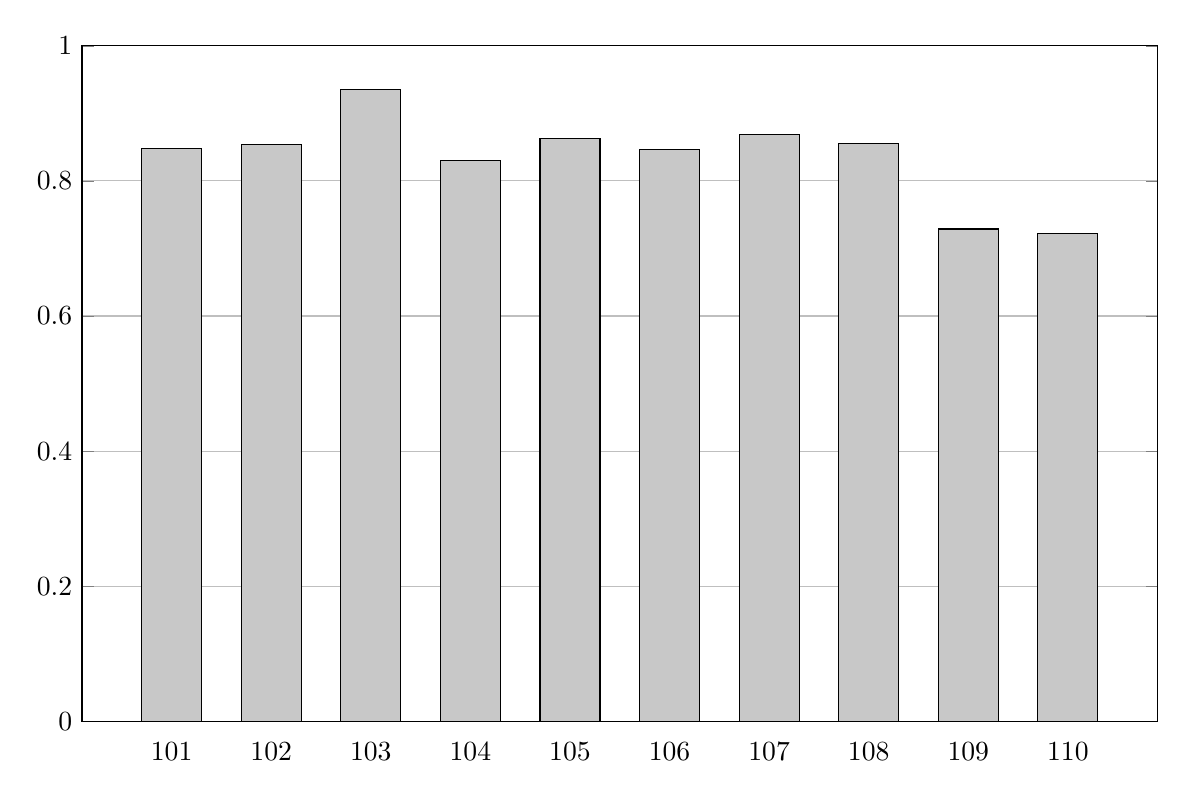
\begin{tikzpicture}
    \begin{axis}[
        width=6in,
	height=4in,
        major x tick style = transparent,
        ybar=2*\pgflinewidth,
        ymajorgrids = true,
        symbolic x coords={101,102,103,104,105,106,107,108,109,110},
        xtick = data,
        scaled y ticks = false,
        enlarge x limits=0.1,
	ymin=0, ymax=1,
        legend cell align=left,
        legend style={
                at={(1.11,0.85)},
                anchor=south east,
                column sep=1ex
        }
    ]
  \addplot[style={bar width=0.3in,fill=wwhite,draw=black}]
            coordinates {	(101,0.8476)
				(102,0.8537)
				(103,0.9353)
				(104,0.8301)
				(105,0.8625)
				(106,0.8465)
				(107,0.8685)
				(108,0.8557)
				(109,0.7288)
				(110,0.7215)	    };
 \end{axis}
\end{tikzpicture}
\end{document}




